\documentclass[a4paper,12pt,french,twocolumn,landscape] {article}

\usepackage[TD]{../../Style}

\renewcommand{\baselinestretch}{1.2}
\geometry{margin=10mm}
\setlength{\columnsep}{20mm}
\pagestyle{empty}

\newcommand{\entetedeux}{
\vspace{-8mm}
Nom: \hfill Prénom: \hfill \
\vspace{4mm}
}

\begin{document}
\entete{~}{\textbf{Questions flash A}}{\premiere ST2S 2}

\entetedeux

\begin{enumerate}

\item Vrai ou faux? Le coefficient multiplicateur lié à une baisse de 30\% est $0,3$.

\vfill

\item Parmi les séquences suivantes, entourer celle ou celles qui peuvent être les premiers termes d'une suite géométrique.

\noindent
2 ; 6 ; 18 \hfill 0 ; 250 ; 500 \hfill 1000 ; 100 ; 10 \hfill -20 ; 12 ; 4

\item Soit $f:x \mapsto 3x-9$ une fonction affine. Entourer le tableau de signes de $f$.

\begin{center}
\begin{tikzpicture}
\tkzTabInit[lgt=1.3,espcl=1.2,deltacl=0.5]{$x$/1, $f(x)$/1}{$-\infty$,3,$+\infty$}
\tkzTabLine{,-,z,+,}
\end{tikzpicture}
\hfill
\begin{tikzpicture}
\tkzTabInit[lgt=1.3,espcl=1.2,deltacl=0.5]{$x$/1, $f(x)$/1}{$-\infty$,6,$+\infty$}
\tkzTabLine{,+,z,-,}
\end{tikzpicture}
\end{center}

\begin{center}
\begin{tikzpicture}
\tkzTabInit[lgt=1.3,espcl=1.2,deltacl=0.5]{$x$/1, $f(x)$/1}{$-\infty$,6,$+\infty$}
\tkzTabLine{,-,z,+,}
\end{tikzpicture}
\hfill
\begin{tikzpicture}
\tkzTabInit[lgt=1.3,espcl=1.2,deltacl=0.5]{$x$/1, $f(x)$/1}{$-\infty$,3,$+\infty$}
\tkzTabLine{,+,z,-,}
\end{tikzpicture}
\end{center}

\item On se donne la fonction $f$ représentée ci-dessous. Donner le maximum de $f$ sur l'intervalle $[1;4]$.

\hfill
\begin{tikzpicture}
\begin{axis}[
styleglobal,
width=0.7*\linewidth,
xmin=-2.5, xmax= 8.5,
ymin=-2.5, ymax=3.5,
xtick distance=1,
ytick distance=1,
minor x tick num=1,
minor y tick num=1,
]
\addplot[styleplot,tension=0.3] plot coordinates{(-2,-1.5) (-0.5,1) (2,1.5) (3,3) (5,1) (6,2) (8,-2)} node[pos=0.72,above] {$\mathscr C_f$} \pointsextremites;
\end{axis}
\end{tikzpicture}

\end{enumerate}
\newpage

\entete{~}{\textbf{Questions flash B}}{\premiere ST2S 2}

\entetedeux

\begin{enumerate}

\item Vrai ou faux? Effectuer une augmentation de 50\% puis à une baisse de 50\% revient à ne rien faire.

\vfill

\item Parmi les séquences suivantes, entourer celle ou celles qui peuvent être les premiers termes d'une suite géométrique.

\noindent
2 ; 6 ; 18 \hfill 0 ; 250 ; 500 \hfill 1000 ; 100 ; 10 \hfill -20 ; 12 ; 4

\vfill

\item Soit $f:x \mapsto 3x-9$ une fonction affine. Compléter le tableau de signes de $f$.

\begin{center}
\begin{tikzpicture}
\tkzTabInit[lgt=1.3,espcl=1.5,deltacl=0.5]{$x$/1, $f(x)$/1}{,,}
\tkzTabLine{,,z,,}
\end{tikzpicture}
\end{center}

\item On se donne la fonction $f$ représentée ci-dessous. Donner le maximum de $f$ sur l'intervalle $[3,5 ; 5]$.

\hfill
\begin{tikzpicture}
\begin{axis}[
styleglobal,
width=0.6\linewidth,
xmin=-1, xmax=7,
ymin=-1, ymax=4,
xtick distance=1,
ytick distance=1,
minor x tick num=1,
minor y tick num=1,
]
\addplot[styleplot,tension=0.3] plot coordinates {(-0.5,1) (2,1.5) (3,3) (5,1) (6.5,2)} node[pos=0.9,below right] {$\mathscr C_f$} \pointsextremites;
\end{axis}
\end{tikzpicture}

\end{enumerate}

\end{document}
